\documentclass[twoside]{book}

% Packages required by doxygen
\usepackage{fixltx2e}
\usepackage{calc}
\usepackage{doxygen}
\usepackage[export]{adjustbox} % also loads graphicx
\usepackage{graphicx}
\usepackage[utf8]{inputenc}
\usepackage{makeidx}
\usepackage{multicol}
\usepackage{multirow}
\PassOptionsToPackage{warn}{textcomp}
\usepackage{textcomp}
\usepackage[nointegrals]{wasysym}
\usepackage[table]{xcolor}

% Font selection
\usepackage[T1]{fontenc}
\usepackage[scaled=.90]{helvet}
\usepackage{courier}
\usepackage{amssymb}
\usepackage{sectsty}
\renewcommand{\familydefault}{\sfdefault}
\allsectionsfont{%
  \fontseries{bc}\selectfont%
  \color{darkgray}%
}
\renewcommand{\DoxyLabelFont}{%
  \fontseries{bc}\selectfont%
  \color{darkgray}%
}
\newcommand{\+}{\discretionary{\mbox{\scriptsize$\hookleftarrow$}}{}{}}

% Page & text layout
\usepackage{geometry}
\geometry{%
  a4paper,%
  top=2.5cm,%
  bottom=2.5cm,%
  left=2.5cm,%
  right=2.5cm%
}
\tolerance=750
\hfuzz=15pt
\hbadness=750
\setlength{\emergencystretch}{15pt}
\setlength{\parindent}{0cm}
\setlength{\parskip}{3ex plus 2ex minus 2ex}
\makeatletter
\renewcommand{\paragraph}{%
  \@startsection{paragraph}{4}{0ex}{-1.0ex}{1.0ex}{%
    \normalfont\normalsize\bfseries\SS@parafont%
  }%
}
\renewcommand{\subparagraph}{%
  \@startsection{subparagraph}{5}{0ex}{-1.0ex}{1.0ex}{%
    \normalfont\normalsize\bfseries\SS@subparafont%
  }%
}
\makeatother

% Headers & footers
\usepackage{fancyhdr}
\pagestyle{fancyplain}
\fancyhead[LE]{\fancyplain{}{\bfseries\thepage}}
\fancyhead[CE]{\fancyplain{}{}}
\fancyhead[RE]{\fancyplain{}{\bfseries\leftmark}}
\fancyhead[LO]{\fancyplain{}{\bfseries\rightmark}}
\fancyhead[CO]{\fancyplain{}{}}
\fancyhead[RO]{\fancyplain{}{\bfseries\thepage}}
\fancyfoot[LE]{\fancyplain{}{}}
\fancyfoot[CE]{\fancyplain{}{}}
\fancyfoot[RE]{\fancyplain{}{\bfseries\scriptsize Generated by Doxygen }}
\fancyfoot[LO]{\fancyplain{}{\bfseries\scriptsize Generated by Doxygen }}
\fancyfoot[CO]{\fancyplain{}{}}
\fancyfoot[RO]{\fancyplain{}{}}
\renewcommand{\footrulewidth}{0.4pt}
\renewcommand{\chaptermark}[1]{%
  \markboth{#1}{}%
}
\renewcommand{\sectionmark}[1]{%
  \markright{\thesection\ #1}%
}

% Indices & bibliography
\usepackage{natbib}
\usepackage[titles]{tocloft}
\setcounter{tocdepth}{3}
\setcounter{secnumdepth}{5}
\makeindex

% Hyperlinks (required, but should be loaded last)
\usepackage{ifpdf}
\ifpdf
  \usepackage[pdftex,pagebackref=true]{hyperref}
\else
  \usepackage[ps2pdf,pagebackref=true]{hyperref}
\fi
\hypersetup{%
  colorlinks=true,%
  linkcolor=blue,%
  citecolor=blue,%
  unicode%
}

% Custom commands
\newcommand{\clearemptydoublepage}{%
  \newpage{\pagestyle{empty}\cleardoublepage}%
}

\usepackage{caption}
\captionsetup{labelsep=space,justification=centering,font={bf},singlelinecheck=off,skip=4pt,position=top}

%===== C O N T E N T S =====

\begin{document}

% Titlepage & ToC
\hypersetup{pageanchor=false,
             bookmarksnumbered=true,
             pdfencoding=unicode
            }
\pagenumbering{alph}
\begin{titlepage}
\vspace*{7cm}
\begin{center}%
{\Large Better Scientific Software }\\
\vspace*{1cm}
{\large Generated by Doxygen 1.8.13}\\
\end{center}
\end{titlepage}
\clearemptydoublepage
\pagenumbering{roman}
\tableofcontents
\clearemptydoublepage
\pagenumbering{arabic}
\hypersetup{pageanchor=true}

%--- Begin generated contents ---
\chapter{Main Page}
\label{index}\hypertarget{index}{}Class relations expressed via an inline dot graph\+: 
\begin{DoxyImageNoCaption}
  \mbox{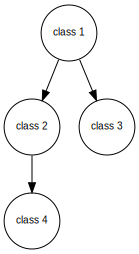
\includegraphics[width=\textwidth,height=\textheight/2,keepaspectratio=true]{dot_inline_dotgraph_1}}
\end{DoxyImageNoCaption}
 Note that the classes in the above graph are clickable (in the H\+T\+ML output). 
\begin{DoxyImageNoCaption}
  \mbox{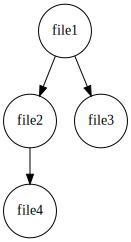
\includegraphics[width=\textwidth,height=\textheight/2,keepaspectratio=true]{dot_grap2}}
\end{DoxyImageNoCaption}
 
\chapter{Category}
\label{md_markdown_category}
\Hypertarget{md_markdown_category}
\input{md_markdown_category}
\chapter{file1}
\label{md_markdown_file1}
\Hypertarget{md_markdown_file1}

\begin{DoxyCode}
#include <iostream>
using namespace std;

python
int main()\{
    cout << "Hello world";
\}
\end{DoxyCode}
 
\chapter{file2}
\label{md_markdown_file2}
\Hypertarget{md_markdown_file2}
\input{md_markdown_file2}
\chapter{file3}
\label{md_markdown_file3}
\Hypertarget{md_markdown_file3}
\input{md_markdown_file3}
\chapter{file4}
\label{md_markdown_file4}
\Hypertarget{md_markdown_file4}

\begin{DoxyCode}
#include <iostream>
using namespace std;


class file2;

int main()\{
    cout << "File4 depends on file2";
\}
\end{DoxyCode}
 
\chapter{This is header}
\label{md_markdown_intro1}
\Hypertarget{md_markdown_intro1}
\input{md_markdown_intro1}
\chapter{Level}
\label{md_markdown_level}
\Hypertarget{md_markdown_level}
\input{md_markdown_level}
\chapter{Level 0}
\label{md_markdown_level0}
\Hypertarget{md_markdown_level0}
\input{md_markdown_level0}
\chapter{Level 1}
\label{md_markdown_level1}
\Hypertarget{md_markdown_level1}

\begin{DoxyImageNoCaption}
  \mbox{\includegraphics[width=\textwidth,height=\textheight/2,keepaspectratio=true]{dot_level1}}
\end{DoxyImageNoCaption}
 
\chapter{Level 2}
\label{md_markdown_level2}
\Hypertarget{md_markdown_level2}
\input{md_markdown_level2}
\chapter{Tags}
\label{md_markdown_tags}
\Hypertarget{md_markdown_tags}
\input{md_markdown_tags}
\chapter{Topic\+: Coding}
\label{md_markdown_topic_coding}
\Hypertarget{md_markdown_topic_coding}
\input{md_markdown_topic_coding}
\chapter{Topic\+: Configuration and building}
\label{md_markdown_topic_configuration_and_building}
\Hypertarget{md_markdown_topic_configuration_and_building}

\begin{DoxyImageNoCaption}
  \mbox{\includegraphics[width=\textwidth,height=\textheight/2,keepaspectratio=true]{dot_topic_configuration_and_building}}
\end{DoxyImageNoCaption}
 
\chapter{Topic\+: Configuration and builds}
\label{md_markdown_topic_configuration_and_builds}
\Hypertarget{md_markdown_topic_configuration_and_builds}
\input{md_markdown_topic_configuration_and_builds}
\chapter{Topic\+: Continuous Integration Testing}
\label{md_markdown_topic_continuous_integration_testing}
\Hypertarget{md_markdown_topic_continuous_integration_testing}

\begin{DoxyImageNoCaption}
  \mbox{\includegraphics[width=\textwidth,height=\textheight/2,keepaspectratio=true]{dot_topic_continuous_integration_testing}}
\end{DoxyImageNoCaption}
 
\chapter{Topic\+: Deployment}
\label{md_markdown_topic_deployment}
\Hypertarget{md_markdown_topic_deployment}
\input{md_markdown_topic_deployment}
\chapter{Topic\+: Development}
\label{md_markdown_topic_development}
\Hypertarget{md_markdown_topic_development}
\input{md_markdown_topic_development}
\chapter{Topic\+: Development Tools}
\label{md_markdown_topic_development_tools}
\Hypertarget{md_markdown_topic_development_tools}
\input{md_markdown_topic_development_tools}
\chapter{Topic\+: Documentation}
\label{md_markdown_topic_documentation}
\Hypertarget{md_markdown_topic_documentation}
\input{md_markdown_topic_documentation}
\chapter{Topic\+: Funding Sources and Programs}
\label{md_markdown_topic_funding_sources_and_programs}
\Hypertarget{md_markdown_topic_funding_sources_and_programs}

\begin{DoxyImage}
\includegraphics[width=\textwidth,height=\textheight/2,keepaspectratio=true]{dot_}
\doxyfigcaption{sources and programs.dot }
\end{DoxyImage}
 
\chapter{Topic\+: Improving Productivity and Sustainability}
\label{md_markdown_topic_improving_productivity_and_sustanability}
\Hypertarget{md_markdown_topic_improving_productivity_and_sustanability}

\begin{DoxyImageNoCaption}
  \mbox{\includegraphics[width=\textwidth,height=\textheight/2,keepaspectratio=true]{dot_topic_improving_productivity_and_sustainability}}
\end{DoxyImageNoCaption}
 
\chapter{Topic\+: Licensing}
\label{md_markdown_topic_licensing}
\Hypertarget{md_markdown_topic_licensing}
\input{md_markdown_topic_licensing}
\chapter{Topic\+: Performance}
\label{md_markdown_topic_performance}
\Hypertarget{md_markdown_topic_performance}
\input{md_markdown_topic_performance}
\chapter{Topic\+: Performance Portability}
\label{md_markdown_topic_performance_portability}
\Hypertarget{md_markdown_topic_performance_portability}

\begin{DoxyImageNoCaption}
  \mbox{\includegraphics[width=\textwidth,height=\textheight/2,keepaspectratio=true]{dot_topic_performance_portability}}
\end{DoxyImageNoCaption}
 
\chapter{Topic\+: Personal Kanban}
\label{md_markdown_topic_personal_kanban}
\Hypertarget{md_markdown_topic_personal_kanban}

\begin{DoxyImageNoCaption}
  \mbox{\includegraphics[width=\textwidth,height=\textheight/2,keepaspectratio=true]{dot_topic_personal_kanban}}
\end{DoxyImageNoCaption}
 
\chapter{Topic\+: Personal Productivity and Sustainability}
\label{md_markdown_topic_personal_productivity_and_sustainability}
\Hypertarget{md_markdown_topic_personal_productivity_and_sustainability}

\begin{DoxyImageNoCaption}
  \mbox{\includegraphics[width=\textwidth,height=\textheight/2,keepaspectratio=true]{dot_topic_personal_productivity_and_sustainability}}
\end{DoxyImageNoCaption}
 
\chapter{Topic\+: Portability}
\label{md_markdown_topic_portability}
\Hypertarget{md_markdown_topic_portability}
\input{md_markdown_topic_portability}
\chapter{Topic\+: Projects and Organizations}
\label{md_markdown_topic_projects_and_organizations}
\Hypertarget{md_markdown_topic_projects_and_organizations}

\begin{DoxyImageNoCaption}
  \mbox{\includegraphics[width=\textwidth,height=\textheight/2,keepaspectratio=true]{dot_topic_projects_and_organizations}}
\end{DoxyImageNoCaption}
 
\chapter{Topic\+: Publication}
\label{md_markdown_topic_publication}
\Hypertarget{md_markdown_topic_publication}
\input{md_markdown_topic_publication}
\chapter{Topic\+: Reliability}
\label{md_markdown_topic_reliability}
\Hypertarget{md_markdown_topic_reliability}
\input{md_markdown_topic_reliability}
\chapter{Topic\+: Reproducibility}
\label{md_markdown_topic_reproducibility}
\Hypertarget{md_markdown_topic_reproducibility}
\input{md_markdown_topic_reproducibility}
\chapter{Topic\+: Requirements}
\label{md_markdown_topic_requirements}
\Hypertarget{md_markdown_topic_requirements}
\input{md_markdown_topic_requirements}
\chapter{Topic\+: Software Development}
\label{md_markdown_topic_software_development}
\Hypertarget{md_markdown_topic_software_development}
\input{md_markdown_topic_software_development}
\chapter{Topic\+: Software Engineering}
\label{md_markdown_topic_software_engineering}
\Hypertarget{md_markdown_topic_software_engineering}
\input{md_markdown_topic_software_engineering}
\chapter{Topic\+: Software Interoperability}
\label{md_markdown_topic_software_interoperability}
\Hypertarget{md_markdown_topic_software_interoperability}
\input{md_markdown_topic_software_interoperability}
\chapter{Topic\+: Software Publishing and Citation}
\label{md_markdown_topic_software_publishing_and_citation}
\Hypertarget{md_markdown_topic_software_publishing_and_citation}

\begin{DoxyImageNoCaption}
  \mbox{\includegraphics[width=\textwidth,height=\textheight/2,keepaspectratio=true]{dot_topic_software_publishing_and_citation}}
\end{DoxyImageNoCaption}
 
\chapter{Topic\+: Strategies for more effective teams}
\label{md_markdown_topic_stategies_for_more_effective_teams}
\Hypertarget{md_markdown_topic_stategies_for_more_effective_teams}
\input{md_markdown_topic_stategies_for_more_effective_teams}
\chapter{Topic\+: Testing}
\label{md_markdown_topic_testing}
\Hypertarget{md_markdown_topic_testing}
\input{md_markdown_topic_testing}
\chapter{Topic\+: Tools}
\label{md_markdown_topic_tools}
\Hypertarget{md_markdown_topic_tools}
\input{md_markdown_topic_tools}
\chapter{Topic\+: Version control}
\label{md_markdown_topic_version_control}
\Hypertarget{md_markdown_topic_version_control}

\begin{DoxyImageNoCaption}
  \mbox{\includegraphics[width=\textwidth,height=\textheight/2,keepaspectratio=true]{dot_topic_version_control}}
\end{DoxyImageNoCaption}
 
\chapter{Topic}
\label{md_markdown_topics}
\Hypertarget{md_markdown_topics}
\input{md_markdown_topics}
\chapter{Namespace Index}
\input{namespaces}
\chapter{File Index}
\section{File List}
Here is a list of all files with brief descriptions\+:\begin{DoxyCompactList}
\item\contentsline{section}{markdown/\hyperlink{intro_8java}{intro.\+java} }{\pageref{intro_8java}}{}
\end{DoxyCompactList}

\chapter{Namespace Documentation}
\input{namespacesubfiles__generator}
\chapter{File Documentation}
\hypertarget{category_8md}{}\section{markdown/category.md File Reference}
\label{category_8md}\index{markdown/category.\+md@{markdown/category.\+md}}

\hypertarget{file1_8md}{}\section{markdown/file1.md File Reference}
\label{file1_8md}\index{markdown/file1.\+md@{markdown/file1.\+md}}

\hypertarget{file2_8md}{}\section{markdown/file2.md File Reference}
\label{file2_8md}\index{markdown/file2.\+md@{markdown/file2.\+md}}

\hypertarget{file3_8md}{}\section{markdown/file3.md File Reference}
\label{file3_8md}\index{markdown/file3.\+md@{markdown/file3.\+md}}

\hypertarget{file4_8md}{}\section{markdown/file4.md File Reference}
\label{file4_8md}\index{markdown/file4.\+md@{markdown/file4.\+md}}

\hypertarget{intro_8java}{}\section{markdown/intro.java File Reference}
\label{intro_8java}\index{markdown/intro.\+java@{markdown/intro.\+java}}
\subsection*{Classes}
\begin{DoxyCompactItemize}
\item 
class {\bfseries B}
\item 
class {\bfseries C}
\end{DoxyCompactItemize}

\hypertarget{intro1_8md}{}\section{markdown/intro1.md File Reference}
\label{intro1_8md}\index{markdown/intro1.\+md@{markdown/intro1.\+md}}

\hypertarget{level_8md}{}\section{markdown/level.md File Reference}
\label{level_8md}\index{markdown/level.\+md@{markdown/level.\+md}}

\hypertarget{level0_8md}{}\section{markdown/level0.md File Reference}
\label{level0_8md}\index{markdown/level0.\+md@{markdown/level0.\+md}}

\hypertarget{level1_8md}{}\section{markdown/level1.md File Reference}
\label{level1_8md}\index{markdown/level1.\+md@{markdown/level1.\+md}}

\hypertarget{level2_8md}{}\section{markdown/level2.md File Reference}
\label{level2_8md}\index{markdown/level2.\+md@{markdown/level2.\+md}}

\input{subfiles__generator_8py}
\hypertarget{tags_8md}{}\section{markdown/tags.md File Reference}
\label{tags_8md}\index{markdown/tags.\+md@{markdown/tags.\+md}}

\hypertarget{topic__coding_8md}{}\section{markdown/topic\+\_\+coding.md File Reference}
\label{topic__coding_8md}\index{markdown/topic\+\_\+coding.\+md@{markdown/topic\+\_\+coding.\+md}}

\hypertarget{topic__configuration__and__building_8md}{}\section{markdown/topic\+\_\+configuration\+\_\+and\+\_\+building.md File Reference}
\label{topic__configuration__and__building_8md}\index{markdown/topic\+\_\+configuration\+\_\+and\+\_\+building.\+md@{markdown/topic\+\_\+configuration\+\_\+and\+\_\+building.\+md}}

\hypertarget{topic__configuration__and__builds_8md}{}\section{markdown/topic\+\_\+configuration\+\_\+and\+\_\+builds.md File Reference}
\label{topic__configuration__and__builds_8md}\index{markdown/topic\+\_\+configuration\+\_\+and\+\_\+builds.\+md@{markdown/topic\+\_\+configuration\+\_\+and\+\_\+builds.\+md}}

\hypertarget{topic__continuous__integration__testing_8md}{}\section{markdown/topic\+\_\+continuous\+\_\+integration\+\_\+testing.md File Reference}
\label{topic__continuous__integration__testing_8md}\index{markdown/topic\+\_\+continuous\+\_\+integration\+\_\+testing.\+md@{markdown/topic\+\_\+continuous\+\_\+integration\+\_\+testing.\+md}}

\hypertarget{topic__deployment_8md}{}\section{markdown/topic\+\_\+deployment.md File Reference}
\label{topic__deployment_8md}\index{markdown/topic\+\_\+deployment.\+md@{markdown/topic\+\_\+deployment.\+md}}

\hypertarget{topic__development_8md}{}\section{markdown/topic\+\_\+development.md File Reference}
\label{topic__development_8md}\index{markdown/topic\+\_\+development.\+md@{markdown/topic\+\_\+development.\+md}}

\hypertarget{topic__development__tools_8md}{}\section{markdown/topic\+\_\+development\+\_\+tools.md File Reference}
\label{topic__development__tools_8md}\index{markdown/topic\+\_\+development\+\_\+tools.\+md@{markdown/topic\+\_\+development\+\_\+tools.\+md}}

\hypertarget{topic__documentation_8md}{}\section{markdown/topic\+\_\+documentation.md File Reference}
\label{topic__documentation_8md}\index{markdown/topic\+\_\+documentation.\+md@{markdown/topic\+\_\+documentation.\+md}}

\hypertarget{topic__funding__sources__and__programs_8md}{}\section{markdown/topic\+\_\+funding\+\_\+sources\+\_\+and\+\_\+programs.md File Reference}
\label{topic__funding__sources__and__programs_8md}\index{markdown/topic\+\_\+funding\+\_\+sources\+\_\+and\+\_\+programs.\+md@{markdown/topic\+\_\+funding\+\_\+sources\+\_\+and\+\_\+programs.\+md}}

\hypertarget{topic__improving__productivity__and__sustanability_8md}{}\section{markdown/topic\+\_\+improving\+\_\+productivity\+\_\+and\+\_\+sustanability.md File Reference}
\label{topic__improving__productivity__and__sustanability_8md}\index{markdown/topic\+\_\+improving\+\_\+productivity\+\_\+and\+\_\+sustanability.\+md@{markdown/topic\+\_\+improving\+\_\+productivity\+\_\+and\+\_\+sustanability.\+md}}

\hypertarget{topic__licensing_8md}{}\section{markdown/topic\+\_\+licensing.md File Reference}
\label{topic__licensing_8md}\index{markdown/topic\+\_\+licensing.\+md@{markdown/topic\+\_\+licensing.\+md}}

\hypertarget{topic__performance_8md}{}\section{markdown/topic\+\_\+performance.md File Reference}
\label{topic__performance_8md}\index{markdown/topic\+\_\+performance.\+md@{markdown/topic\+\_\+performance.\+md}}

\hypertarget{topic__performance__portability_8md}{}\section{markdown/topic\+\_\+performance\+\_\+portability.md File Reference}
\label{topic__performance__portability_8md}\index{markdown/topic\+\_\+performance\+\_\+portability.\+md@{markdown/topic\+\_\+performance\+\_\+portability.\+md}}

\hypertarget{topic__personal__kanban_8md}{}\section{markdown/topic\+\_\+personal\+\_\+kanban.md File Reference}
\label{topic__personal__kanban_8md}\index{markdown/topic\+\_\+personal\+\_\+kanban.\+md@{markdown/topic\+\_\+personal\+\_\+kanban.\+md}}

\hypertarget{topic__personal__productivity__and__sustainability_8md}{}\section{markdown/topic\+\_\+personal\+\_\+productivity\+\_\+and\+\_\+sustainability.md File Reference}
\label{topic__personal__productivity__and__sustainability_8md}\index{markdown/topic\+\_\+personal\+\_\+productivity\+\_\+and\+\_\+sustainability.\+md@{markdown/topic\+\_\+personal\+\_\+productivity\+\_\+and\+\_\+sustainability.\+md}}

\hypertarget{topic__portability_8md}{}\section{markdown/topic\+\_\+portability.md File Reference}
\label{topic__portability_8md}\index{markdown/topic\+\_\+portability.\+md@{markdown/topic\+\_\+portability.\+md}}

\hypertarget{topic__projects__and__organizations_8md}{}\section{markdown/topic\+\_\+projects\+\_\+and\+\_\+organizations.md File Reference}
\label{topic__projects__and__organizations_8md}\index{markdown/topic\+\_\+projects\+\_\+and\+\_\+organizations.\+md@{markdown/topic\+\_\+projects\+\_\+and\+\_\+organizations.\+md}}

\hypertarget{topic__publication_8md}{}\section{markdown/topic\+\_\+publication.md File Reference}
\label{topic__publication_8md}\index{markdown/topic\+\_\+publication.\+md@{markdown/topic\+\_\+publication.\+md}}

\hypertarget{topic__reliability_8md}{}\section{markdown/topic\+\_\+reliability.md File Reference}
\label{topic__reliability_8md}\index{markdown/topic\+\_\+reliability.\+md@{markdown/topic\+\_\+reliability.\+md}}

\hypertarget{topic__reproducibility_8md}{}\section{markdown/topic\+\_\+reproducibility.md File Reference}
\label{topic__reproducibility_8md}\index{markdown/topic\+\_\+reproducibility.\+md@{markdown/topic\+\_\+reproducibility.\+md}}

\hypertarget{topic__requirements_8md}{}\section{markdown/topic\+\_\+requirements.md File Reference}
\label{topic__requirements_8md}\index{markdown/topic\+\_\+requirements.\+md@{markdown/topic\+\_\+requirements.\+md}}

\hypertarget{topic__software__development_8md}{}\section{markdown/topic\+\_\+software\+\_\+development.md File Reference}
\label{topic__software__development_8md}\index{markdown/topic\+\_\+software\+\_\+development.\+md@{markdown/topic\+\_\+software\+\_\+development.\+md}}

\hypertarget{topic__software__engineering_8md}{}\section{markdown/topic\+\_\+software\+\_\+engineering.md File Reference}
\label{topic__software__engineering_8md}\index{markdown/topic\+\_\+software\+\_\+engineering.\+md@{markdown/topic\+\_\+software\+\_\+engineering.\+md}}

\hypertarget{topic__software__interoperability_8md}{}\section{markdown/topic\+\_\+software\+\_\+interoperability.md File Reference}
\label{topic__software__interoperability_8md}\index{markdown/topic\+\_\+software\+\_\+interoperability.\+md@{markdown/topic\+\_\+software\+\_\+interoperability.\+md}}

\hypertarget{topic__software__publishing__and__citation_8md}{}\section{markdown/topic\+\_\+software\+\_\+publishing\+\_\+and\+\_\+citation.md File Reference}
\label{topic__software__publishing__and__citation_8md}\index{markdown/topic\+\_\+software\+\_\+publishing\+\_\+and\+\_\+citation.\+md@{markdown/topic\+\_\+software\+\_\+publishing\+\_\+and\+\_\+citation.\+md}}

\hypertarget{topic__stategies__for__more__effective__teams_8md}{}\section{markdown/topic\+\_\+stategies\+\_\+for\+\_\+more\+\_\+effective\+\_\+teams.md File Reference}
\label{topic__stategies__for__more__effective__teams_8md}\index{markdown/topic\+\_\+stategies\+\_\+for\+\_\+more\+\_\+effective\+\_\+teams.\+md@{markdown/topic\+\_\+stategies\+\_\+for\+\_\+more\+\_\+effective\+\_\+teams.\+md}}

\hypertarget{topic__testing_8md}{}\section{markdown/topic\+\_\+testing.md File Reference}
\label{topic__testing_8md}\index{markdown/topic\+\_\+testing.\+md@{markdown/topic\+\_\+testing.\+md}}

\hypertarget{topic__tools_8md}{}\section{markdown/topic\+\_\+tools.md File Reference}
\label{topic__tools_8md}\index{markdown/topic\+\_\+tools.\+md@{markdown/topic\+\_\+tools.\+md}}

\hypertarget{topic__version__control_8md}{}\section{markdown/topic\+\_\+version\+\_\+control.md File Reference}
\label{topic__version__control_8md}\index{markdown/topic\+\_\+version\+\_\+control.\+md@{markdown/topic\+\_\+version\+\_\+control.\+md}}

\input{topics_8md}
%--- End generated contents ---

% Index
\backmatter
\newpage
\phantomsection
\clearemptydoublepage
\addcontentsline{toc}{chapter}{Index}
\printindex

\end{document}
